% Shared section: used by paper-ieee.tex, paper-lncs.tex and report.tex.
% Use \sect / \subsect for headings (see README), never \section directly.

\iffull
\sect{Prospective Validation Protocol}\label{prospective-validation-protocol}
\else
\sect{Future Work}\label{prospective-validation-protocol}
\fi

\iffull
This section describes planned work; none of these experiments has been run yet. The first step is to freeze everything that affects the result: model files, label versions, source groups, exclusions, thresholds, matching rules and how unavailable input is counted. Before any headline comparison, the full event logs for the current model and the pinch-out data should be recovered.
\else
Three studies come next; none has been run yet. First, with models, labels and thresholds frozen in advance, compare IMU-only, PPG-only and fused inputs, rolling against median scaling, and the CNN against engineered-feature trees on the same corrected data. Second, test generalisation with multiple participants across new days and strap refits, holding out whole participants for user-independent claims. Third, run a counterbalanced task comparing look--pinch--turn with a conventional volume control, with fault trials and a latency breakdown, and repeat the selection task inside an AR/VR headset, comparing its camera pinch, the watch pinch and both combined.
\fi

\iffull
\begin{widefigure}
\centering
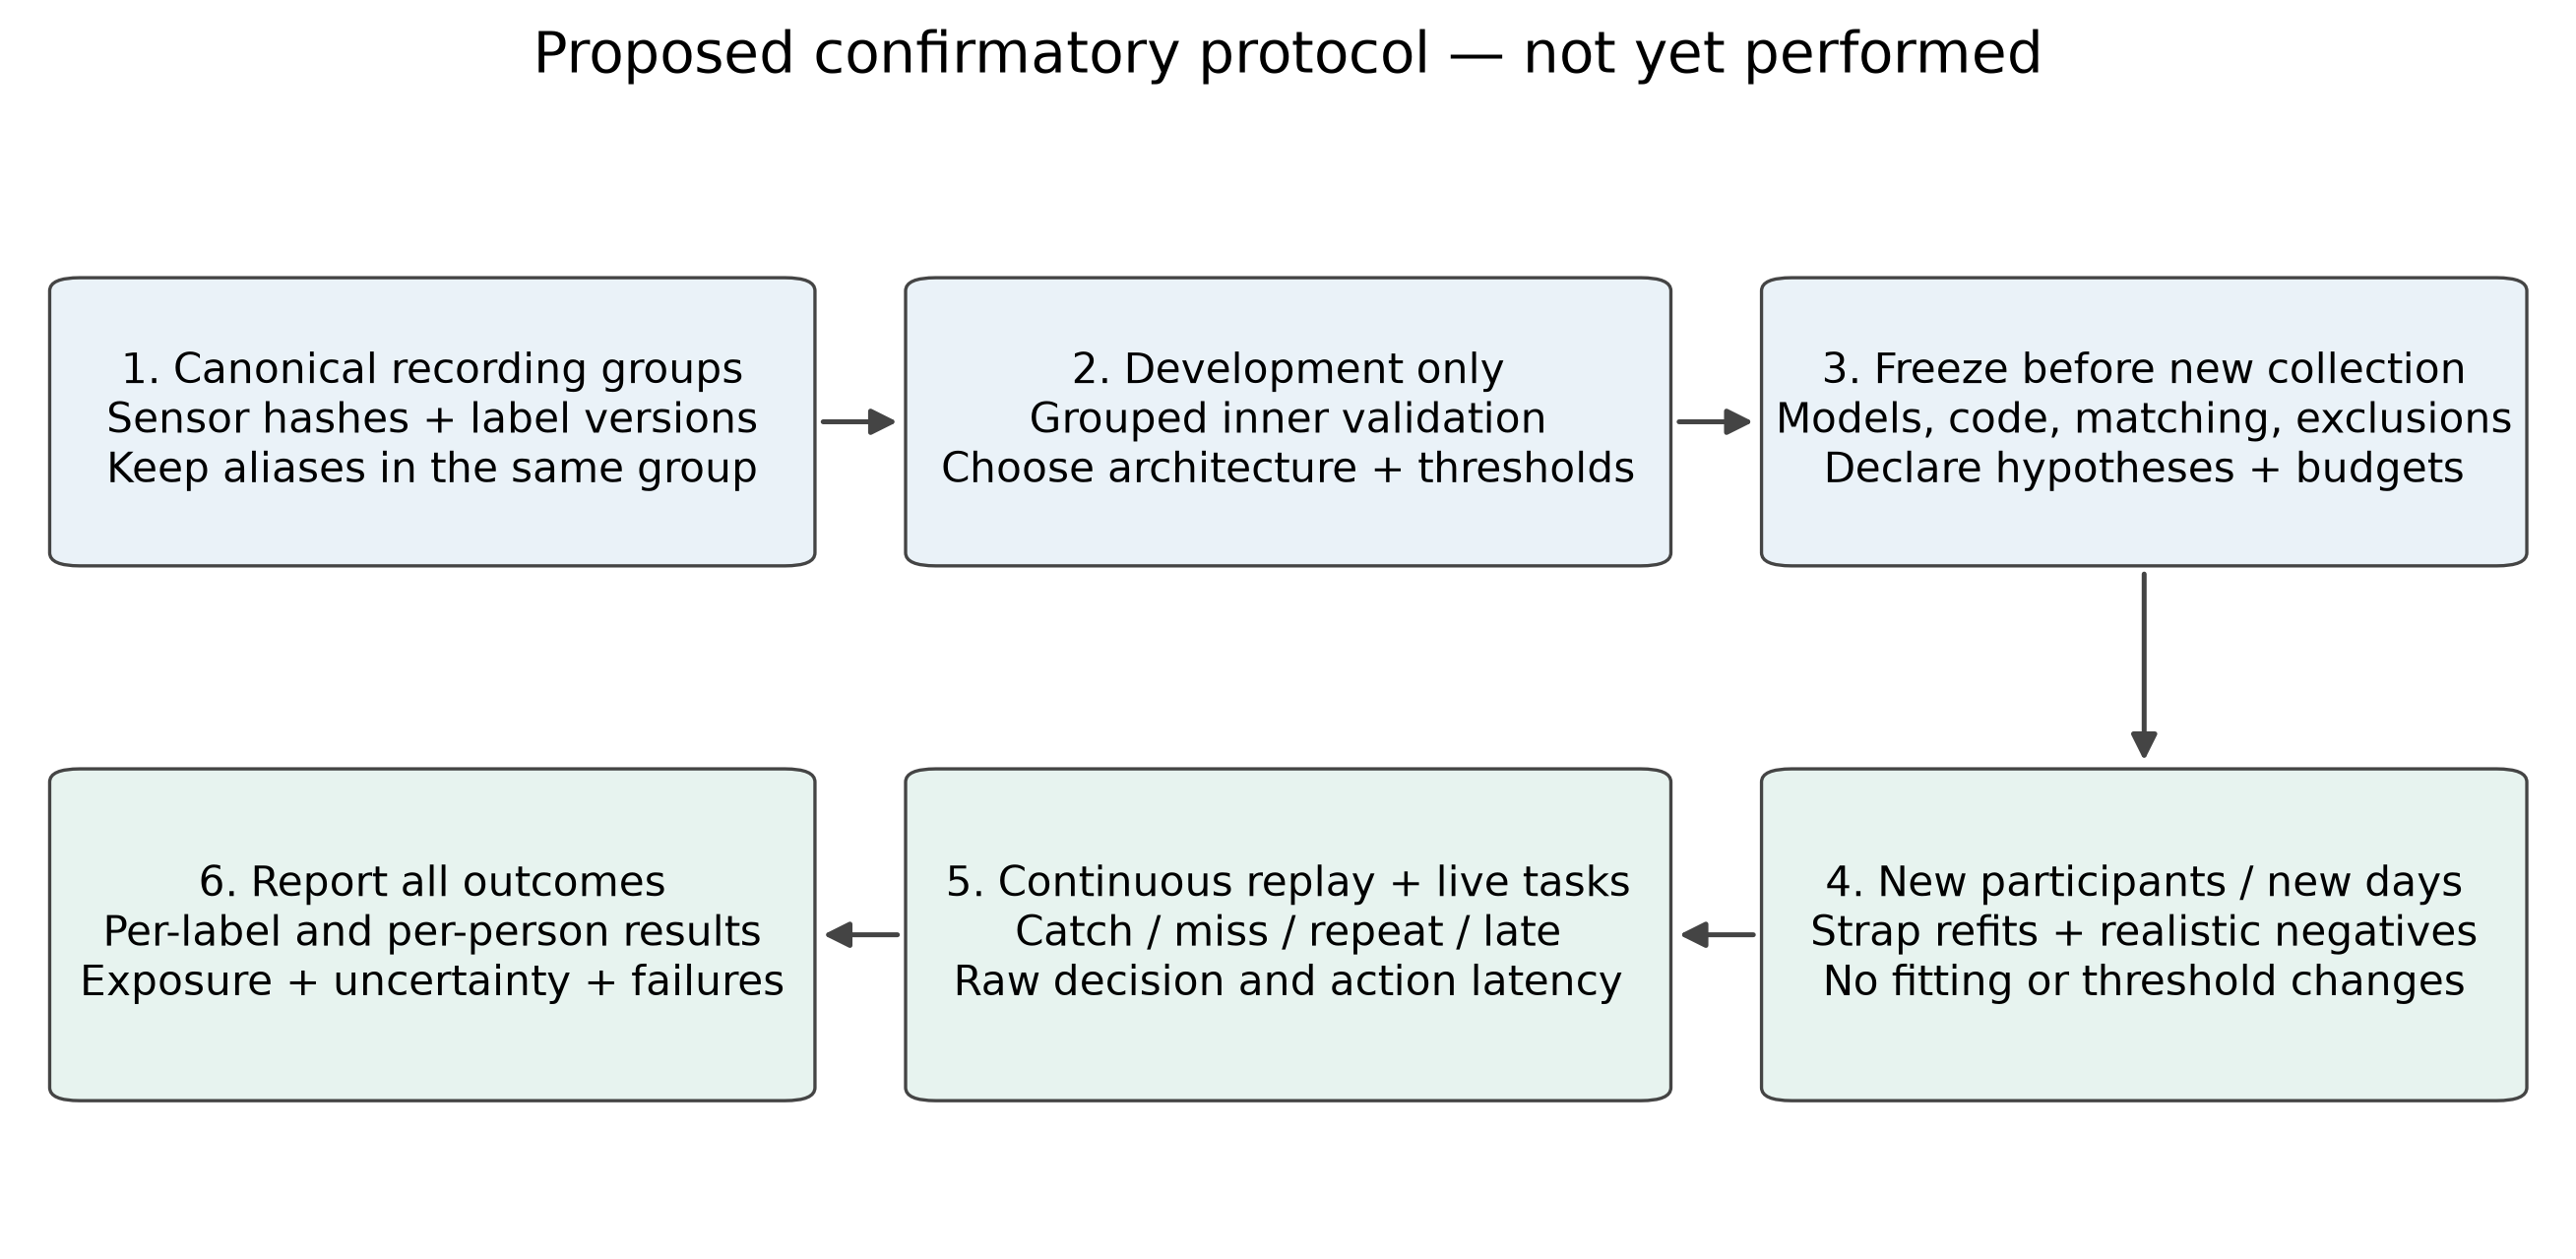
\includegraphics[width=1\linewidth,height=\textheight,keepaspectratio,alt={Proposed development, freeze, prospective collection and continuous/live evaluation sequence.}]{figures/prospective-protocol.png}
\caption{Planned confirmatory workflow: develop, freeze, collect new data, then evaluate continuously and in live use. None of these stages has been carried out yet.}\label{fig-prospective}
\end{widefigure}
\fi

\iffull
\subsect{Matched sensing and preprocessing comparisons}\label{matched-sensing-and-preprocessing-comparisons}
\fi

\iffull
The smallest useful ablation compares IMU-only, PPG-only and fused inputs on the same corrected source groups, then rolling against median scaling, then the CNN against the engineered-feature trees. All variants should share the selection procedure, false-activation target, input rate, exclusions and matching rules. Each may have its own threshold, chosen the same way on development data and never on test data. Synthetic splices are useful, but real pinches after real movement should be tested as well.
\fi

\iffull
\subsect{Personalisation and generalisation}\label{personalisation-and-generalisation}
\fi

\iffull
Different claims need different splits. A personalised claim needs each person's frozen model tested on new days and after the strap is refitted. A user-independent claim needs whole participants held out. Few-shot adaptation needs a calibration block kept separate from the later test. The number of participants and the amount of exposure should be set from pilot variation and the precision we want. New sessions should include ordinary keyboard and mouse use, wrist turns, different arm support and strap fit, and the quiet conditions the interaction assumes. Pinching while the hand moves should be reported separately if it falls outside the intended still-hand use.
\fi

\iffull
\subsect{Interaction and physical fault trials}\label{interaction-and-physical-fault-trials}
\fi

\iffull
A counterbalanced task should compare look--pinch--turn with a conventional volume control, using set practice, target and timeout rules. We would measure completion time, final error, retries, missed grabs and releases, unintended actions, and discomfort and workload. Fault trials should cover stale signals, disconnection and reconnection, the head leaving the target, model replacement and a release while a volume write is still queued. Latency should be broken down into sensing, receipt, scoring, event emission, policy acceptance and the completed output, with clock uncertainty and unavailable intervals reported.
\fi

\iffull
\subsect{Testing in a headset}\label{testing-in-a-headset}
\fi

\iffull
A natural next step is to repeat the selection task inside an AR or VR headset, using the headset's own head or eye tracking for targeting and the watch for pinch-in and pinch-out. Useful comparisons would be the headset's built-in camera pinch alone, the watch pinch alone, and both combined, including trials with the hand deliberately kept out of the cameras' view. The same event-level measures (recall, false activations per hour of no-gesture time, latency) would let the results be compared directly with the desktop study.

\fi